% !TEX root = ../latex-faq-cn.tex
% Copyright (C) 2018 by latexstudio <http://www.latexstudio.net>
%
% This program is free software: you can redistribute it and/or modify
% it under the terms of the GNU General Public License as published by
% the Free Software Foundation, either version 3 of the License, or
% (at your option) any later version.
%
% This program is distributed in the hope that it will be useful,
% but WITHOUT ANY WARRANTY; without even the implied warranty of
% MERCHANTABILITY or FITNESS FOR A PARTICULAR PURPOSE.  See the
% GNU General Public License for more details.
%
% You should have received a copy of the GNU General Public License
% along with this program.  If not, see <http://www.gnu.org/licenses/>.
%

\section{文档编辑}


\faq{\LaTeXTeX{} 教程}{latex-tex-tutorial}
lshort-zh 是一本比较薄的针对中文用户的 \LaTeX{} 入门教程,该教程已在发行版中,用户可以在命令行中执行
\begin{verbatim}
  texdoc lshort-zh
\end{verbatim}
来查阅。 \LaTeX wikibook 是
% \href{https://www.latex-project.org/help/books/}{https://www.latex-project.org/}
\url{https://www.latex-project.org/help/books/} 中列出的 \TeX{} and \LaTeX{} Books 之一,用户可访问
\url{https://en.wikibooks.org/wiki/LaTeX} 进行查阅。
除此之外,用户还可以购买胡伟、刘海洋等编著书籍,这里不再赘述。


\faq{关于 \LaTeX{} 的书籍}{latex-books}
\begin{itemize}
  \item \LaTeX{} 入门,刘海洋, 电子工业出版社;
  \item \LaTeX{2$\varepsilon$} 完全学习手册(第 2 版),胡伟,清华大学出版社;
  \item \LaTeX{} 入门与提高(第二版) ,陈志杰等,高等教育出版社(注:此书出版逾十年,部分内容已经过时);
  \item \LaTeX{} Beginner's Guide, Stefan Kottwit, Packt Publishing.
\end{itemize}


\faq{\LaTeX{} 支持中文有哪些方式,如何选择}{latex-chinese-how-to-choose}
历史上,\LaTeX{} 支持中文的方式包括中西文点点通、天元、CCT、CJK 等。目前流行的方式是使用 \CTeX{} 宏集,详情请见
\url{https://mirrors.tuna.tsinghua.edu.cn/CTAN/language/chinese/ctex/ctex.pdf}


\faq{关于教程,用户比较容易获取的有两个:lshort 和 \LaTeX{} wikibook。}{lshort-latex-wikibook}


\faq{关于\TeX{}, Plain \TeX{} 及相关书籍}{tex-plain-tex-books}


\faq{关于类型的书籍}{kind-related-books}


\faq{关于其他TeX相关事项的书籍}{other-tex-books}


\faq{工具包文档}{package-document}
每个工具包自带的文档是最全面最权威的文档,一般可以通过 texdoc
命令+工具包名的方式找到相应工具包的文档。
一些常用的工具包有不少爱好者写了自己使用过程中的经验,也可以找来看看。


\faq{可免费提供的 \LaTeXTeX{} 书籍}{free-latex-tex-books}
\begin{itemize}
  \item \LaTeX{} 常用数学符号
  \item \LaTeX{} Note 包太雷
  \item 一份不太简短的 \LaTeX{2e} 介绍
  \item \TeX{} Live 指南 2018
\end{itemize}


\faq{获取在线帮助}{gain-online-help}
一般资料可以去 wikibook 上面查询,网址是
\url{https://en.wikibooks.org/wiki/LaTeX}。
提问可以先到 \LaTeX{} Stack Exchange 看看,网址是
\url{https://tex.stackexchange.com/}。


\faq{如何提出问题}{how-to-ask-questions}

在问问题的时候,要先自己尝试,先问自己如何解决,清晰有效的组织自己想问的问题,究竟想表达什么?没有人会为你不知所谓的问题
浪费时间,就算有人愿意理你,也会因为你的问题不清晰甚至完全无效的问题而伤透脑筋,为了自己,也为了别人,建议大家可以参考下
\href{https://www.jianshu.com/p/f96aa7f7bf59}{《提问的艺术》}这篇文字,清晰有效的提出自己的问题。迷你范例(MWE)
是为别人帮助解决你的问题提供最大化便利的有效手段之一。

最后,需要强调的是,我们愿意在我们的能力范围内为你的问题进行讨论,尽全力帮你解决问题,但这并不是我们的义务,应当尊重别人
拒绝提供帮助的权利。另外,在 QQ 群提出问题所使用的代码最好代码粘贴的网站,如
\href{https://paste.ubuntu.com/}{Ubuntu Pastebin}
暂存,避免刷屏,影响效率。


\faq{如何制作一个迷你范例(MWE)}{how-to-make-MWE}
迷你范例即最小工作示例,英文简称 MWE,以下内容摘自刘海洋的《\LaTeX{} 入门》。

最小工作示例就是一个精简到最小长度的、可以说明所需问题的 \TeX{} 源文件。一方面,最小工作示例应该是一个完整的、可以直接
编译的文件,利用示例可以方便地再现遇到的问题,不需要添加额外的代码;另一方面,示例文件应该尽可能地短小(一个典型的 MWE
一般不超过 10 行),不包含额外的文件,也没有与问题无关的文字代码干扰相对错误的分析。完整的 MWE 应当包括如下信息:
\begin{itemize}
  \item 编译环境,至少应当包括使用的操作系统(如 Windows,macOS,Ubuntu)、安装的发行版(如 \CTeX{},\TeX{} Liv
  e,\MacTeX{} )和使用的集成开发环境(IDE)或编辑器(如 WinEdit,TeXstudio,TeXshop)
  \item 完整的编译命令,如使用的排版引擎(如 \LaTeX{},\XeLaTeX{})
  \item 源文件使用的编码,不同的编辑器的默认编码设置不同,没有事先声明可能会造成复现 bug 困难或出现其他 bug
  \item 完整的代码,但应尽量删除与错误无关的部分,即保证代码可以直接运行的前提下,删除所有与错误部分无关的内容和信息,
  足以重现出现的错误信息和问题即可。不要截图!使别人可以直接复制粘贴你的代码到编译器中,直接重现问题,而不是将时间浪费在
  码字上
  \item 编译错误信息,或你发现与预期不符的 PDF 效果
  \item 如使用了模板,还需附上模板的相关信息,如下载链接和使用说明
\end{itemize}


\faq{学习如何撰写 \LaTeX{} 类及工具包}{learn-how-to-write-latex-and-tools}

可以用命令行使用 |texdoc| 查看 clsguide,dtxtut,macros2e;classes,source2e,The TeXBook;expl3,interface3,
l3styleguide,source3(参考自\href{https://www.zhihu.com/question/27017364}{知乎})。以及《\LaTeX{2e}
文类和宏包学习手册》(胡伟,清华大学出版社)。


\faq{MetaFont 和 MetaPost 教程}{metafont-metapost-tutorial}


\faq{在线介绍:\LaTeX{}}{}


\faq{在线介绍:Plain \TeX{}}{}


\faq{如何让参考文献满足国标GB7714-2015样式要求}{how-to-reference-GB}

有两种比较简单的方式。
\begin{itemize}
  \item 利用 biblatex,一个典型示例如下
  \begin{verbatim}
    \documentclass{ctexart}
      \usepackage[backend=biber,style=gb7714-2015]{biblatex}
      \addbibresource{bibfilename.bib}
      \begin{document}
        引用文献\cite{bibkey1,bibkey2}
        \printbibliography
      \end{document}
    \end{verbatim}
  \item 利用 biblatex,一个典型示例如下
  \begin{verbatim}
    \documentclass{ctexart}
      \usepackage{gbt7714}
      \begin{document}
        引用文献\cite{bibkey1,bibkey2}
        \bibliography{bibfilename}
      \end{document}
  \end{verbatim}
\end{itemize}


\faq{专家邮件列表}{}


\faq{Pic\TeX{} 手册}{}


\faq{基于 \TeX{} 系统的教程}{}


\faq{排版教程}{}


\faq{关于 \TeX{} 的 Wiki 书籍}{tex-wiki-books}

\LaTeX{} wikibook 是 \url{https://www.latex-project.org/} 中列出的 \TeX{} and \LaTeX{} Books 之一,用户
可访问 \url{https://en.wikibooks.org/wiki/LaTeX} 进行查阅。


\faq{如何找到\ldots{}符号:}{how-to-find-symbols}
%
%
在 \LaTeX{} 中插入符号主要有两种思路。一种方式是加载符号宏包,利用宏包提供的命令插入符号;而对于 \XeTeX{} 引擎,目前
使用的多为 Unicode 编码的字体,直接加载 Unicode 字体,插入 Unicode 符号也是一种很好的办法。下面分别介绍:
\begin{itemize}
  \item 加载符号宏包:\emph{The Comprehensive LATEX Symbol List} 收录了上万文本或数学符号,在命令行中键入
  \begin{verbatim}
    texdoc symbols-a4
  \end{verbatim}
  即可打开该文档。此外,\url{http://detexify.kirelabs.org/classify.html}提供了手写识别前述文档中所有符号的功能,
  十分便捷,它可直接符号所在宏包。在 macOS 下可以直接使用 detexify 的 app。另外
  \url{https://webdemo.myscript.com/views/main/math.html}可将手写公式转化为 \LaTeX{} 或 MathML 代码
  \item 插入Unicode符号:可以从各种Unicode码表或字符映射表中找到所需要的符号,查出其编码,加载支持该码位的字体,
  直接在编辑器中输入该符号即可。如果符号在源代码编辑器中无法正常显示,还可以使用\LaTeX{}的 |symbol| 命令输入。
  |symbol| 命令的具体用法是
  \begin{verbatim}
    \symbol{<十进制编码>}
    \symbol{"<十六进制编码>}
    \symbol{'<八进制编码>}
    \symbol{`<字符形式(特殊符号须加转义符 \ )>}
  \end{verbatim}
\end{itemize}

如果使用的TeXstudio软件想要查找某个符号,那么还可以拓展以下2个便捷的方式:
\begin{itemize}
  \item 如下图点开1处的符号,再在2处选择符号类型,缩小查找范围,有运算符、关系、箭头、分隔符、Greek、Cyrillic等,再
  点击需要的符号加入到数学环境中去这样就插入完成了。

  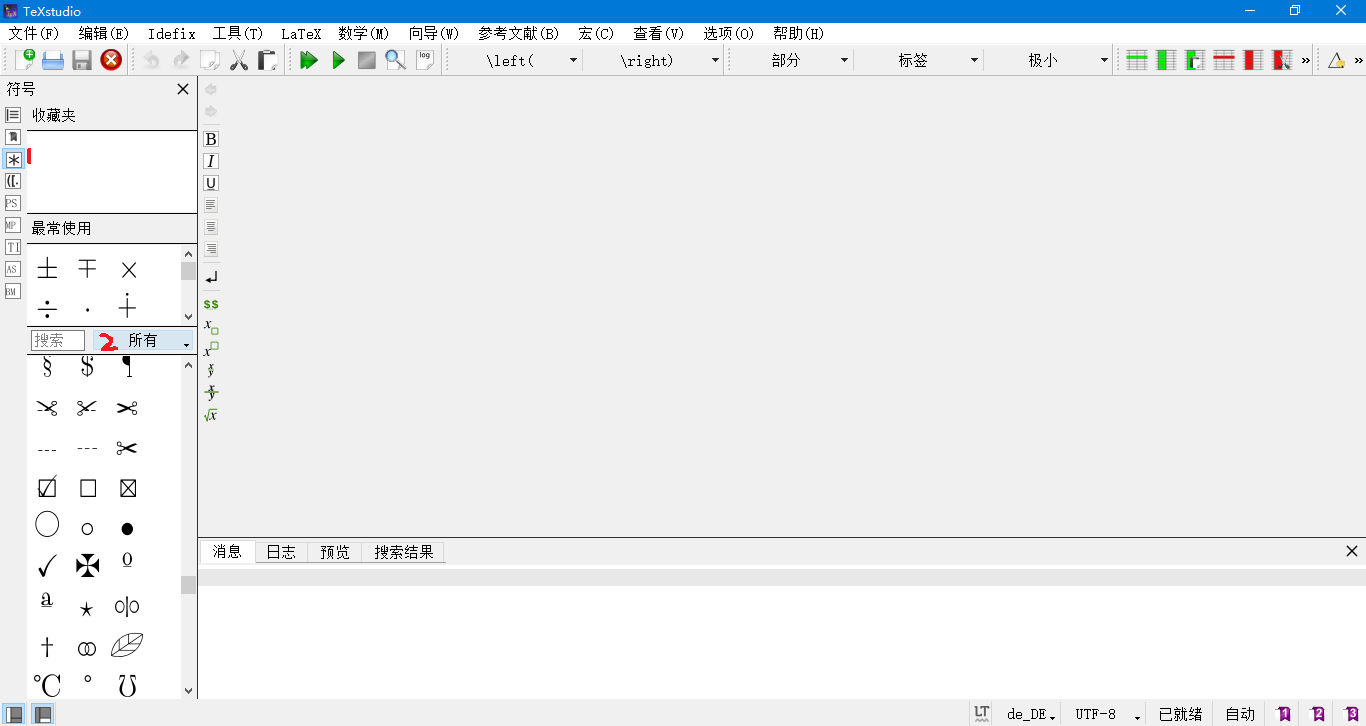
\includegraphics[width=0.9\textwidth]{include/images/5.png}
  \item 也可以手动输入,识别率不是特别高,可能需要多输入几次才会出来。设置如下:向导$\rightarrow$数学助手,手写输入完
  之后插入即可。

  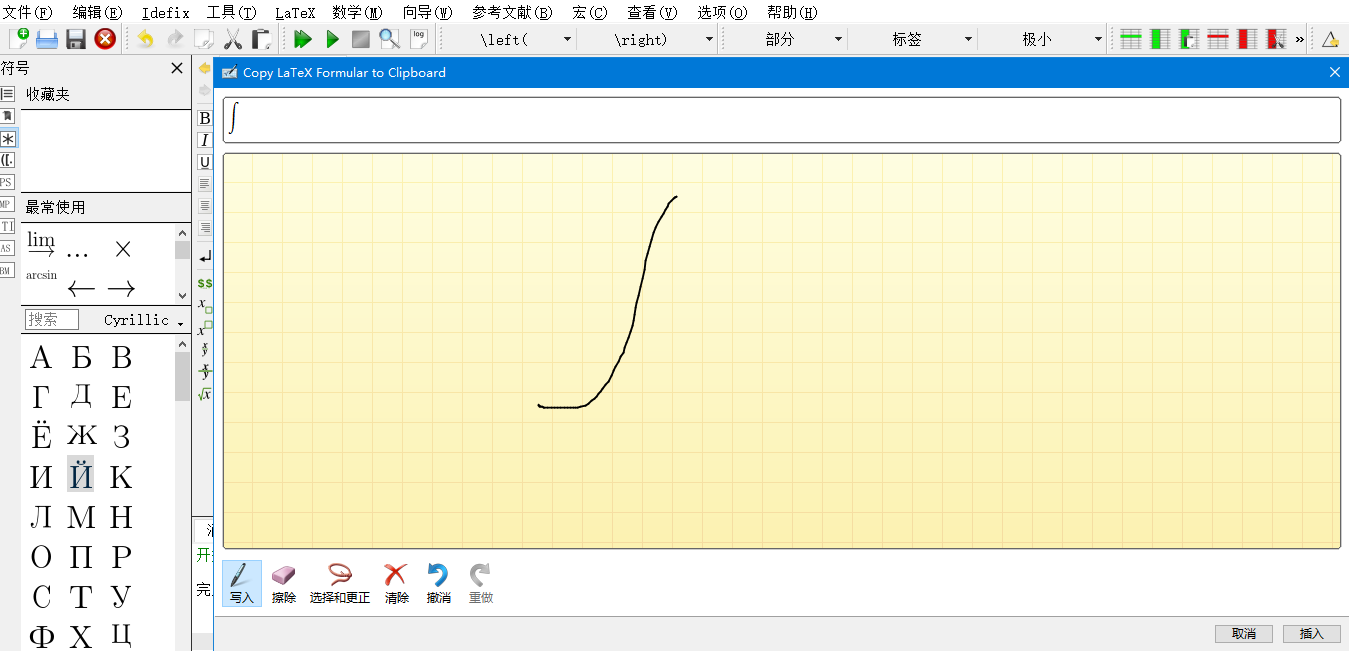
\includegraphics[width=0.9\textwidth]{include/images/image.png}
\end{itemize}


\faq{如何找到 FAQs}{}


\faq{如何控制章节编号的深度}{how-to-control-section-depth}

\LaTeX{} 标准文档类对章节划分了层级:
\begin{itemize}
  \item 在 article 文档类里 part 为0,section 为1,依此类推;
  \item 在 report/book 文档类里 part 为 $-1$,chapter 为0,section 为1,等等。
\end{itemize}

secnumdepth 计数器控制章节编号的深度,如果章节的层级大于secnumdepth,那么章节的标题、在目录和页眉页脚的标题都不编号
(照常生成目录和页眉页脚),章节计数器也不计数。可以用 |setcounter| 命令设置 secnumdepth 为较大的数使得层级比较深的
章节也编号,如设置为4令 |paragraph| 也编号;或者设置一个较小的数以取消编号,如设置为-1 令 |chapter| 不编号。
后者是生成不编号的章节的一个妙招,免去了手动使用 |addcontentsline| 和 |markboth| 的麻烦。
secnumdepth 计数器在 article 文档类里默认为3(subsubsection一级);在 report 和 book 文档类里默认为
2(subsection 一级)。

下面给出一个具体的例子:

\begin{verbatim}
  \documentclass{book}
  \setcounter{secnumdepth}{4}
  \begin{document}
    \part{part}
    \chapter{chapter}
    \section{section}
      \subsection{subsection}
      \subsubsection{subsubsection}
        \paragraph{paragraph}
  \end{document}
\end{verbatim}

控制目录页排版显示深度可以使用 |\setcounter{tocdepth}{2}|,此命令表示显示到三级标题。关于此问题的具体介绍可以参考
\href{https://blog.csdn.net/RobertChenGuangzhi/article/details/50480856}{该网页}。


\faq{如何下载 arXiv 上面的 \TeX{} 源文件}{how-to-download-arxiv-tex}
先访问 arXiv 上面的文章,在右边找到 Downloads $\rightarrow$ Other formats,点击进入下载页,点击 Download source。
将文件下载到本地后,重命名文件,文件后缀名是 .tar.gz。接下来解压缩 .tar.gz 文件,即可获得 \TeX{} 源文件。


\faq{Windows 系统下用 TeXstudio 打开中文编写的源文件遇到乱码怎么办}{windows-texstudio-chinese-GBK}

最简单的方法是借助 Notepad++ 等编辑器将文件转码为 UTF-8。如果没有 noteapd++,也可以直接使用 TeXstudio。
这里我们默认文件的编码是 GB2312。首先打开文件,在 TeXstudio 右下角找到 encoding 位置的内容,
有时系统显示为 ISO-8859-1。点击那里,进入 More encodings,在列表中点击 GB2312,然后点击按钮 view with。
正常来讲,乱码应该都会消失。 接下来,继续进入 More encodings,在列表中点击 UTF-8,然后点击按钮 change to。
经过这些操作,源文件就重新变成了 UTF-8 编码。


\faq{如何在listing抄录环境中显示公式}{how-to-listing-show-equations}

有时对抄录环境中的代码进行说明时,要用显示公式,这时只要进选项texcl设为true即可。

\begin{verbatim}
  \begin{lstlisting}[
    numbers=left,
    upquote=true,
    basicstyle=\ttfamily,
    texcl=true,
    language=Python
    ]
    #Generates Graphs $G^{(12)} ---  G^{(17)}$
    sGL6=['E@QW', 'EHQW', 'E@`w', 'E@]o', 'E@Rw', 'EAMw']
    GL=[Graph(s) for s in sGL6]
    \end{lstlisting}
\end{verbatim}
%  
%  % \begin{figure}
%  % \centering
%  % \includegraphics{https://images-cdn.shimo.im/LttXT6sECbcak9Qi/image.png!thumbnail}
%  % \caption{图片}
%  % \end{figure}
%  

或者设置mathescape~选项为true。

\begin{verbatim}
  \begin{lstlisting}[mathescape=true]
    if foo
    list= { $S_1,S_2,S_3$ }
  \end{lstlisting}
\end{verbatim}


\faq{能不能介绍一下排版试卷的方法与技巧,比如选择题,密封线设置等。}{how-to-latex-papers}


\faq{一个文档,如何在不同部分使用不同的页眉页脚}{how-to-set-different-geometry}

参考 geometry 宏包的自定义命令。比较常用的有如下四个命令
\begin{verbatim}
  \newgeometry{<options>}
  \restoregeometry
  \savegeometry{<name>}
  \loadgeometry{<name>}
\end{verbatim}
具体可参见该宏包的说明文档。


\faq{如何给中文文本加注音符号?}{how-to-pinyin}

xpinyin 宏包。


\faq{在book类文档中边注用什么宏包?边注的宽度能调整吗?}{book-geometry}


\faq{如何使用ctex相关类或者宏包制定章节样式,目录样式?}{ctex-tableofcontents}


\faq{如何给章节标题,目录列表加盒子边框?}{}


\faq{如何使用带圈数字?}{how-to-use-circle-number}

\begin{verbatim}
  \begin{enumerate}
    \def\labelenumi{\arabic{enumi}.}
    \setcounter{enumi}{7}
\end{verbatim}


\faq{如何改变列表标签样式,行距,缩进等各种相关间距?}{how-to-change-list-style}

enumitem 宏包


\faq{换行与换段的区别,有几种方式?}{change-line-paragraph}

换行是 |\\| 换段是 |\par|,或者空一行。
换行与分段最大的区别在于语义上是否形成一段完整的阐述、叙述,多读两遍你写的文字,如果你觉得问题没有叙述完,那么应该用换行,
反之则应该用分段。


\faq{在使用较早版本的CTeX里面附带的WinEdit出现打不开UTF-8编码文档的情况,如何处理?}{early-version-ctex-winedit-utf8}

使用记事本之类文本编辑器打开,转换编码方式另存一份即可。有时候需要注意BOM问题,一般没啥问题。


\faq{如何改变计数器样式为中文数字、罗马数字、阿拉伯数字或拉丁字母?}{how-to-change-listing-number}

可以通过重定义命令的方式修改默认的计数器样式,例如
\begin{verbatim}
  \renewcommand{\thechapter}{\Roman{chapter}}
\end{verbatim}
会将章序号计数器改为大写罗马数字计数形式。更多对应关系如下所示:

\begin{table}[h]
  \centering
  \begin{tabular}{cc}
    |\arabic| & 阿拉伯数字 \\
    |\alph| & 小写英文字母,数值应小于27 \\
    |\Alph| & 大写英文字母,数值应小于27 \\
    |\chinese| & 中文小写数字,需要调用\CTeX{}宏包 \\
    |\roman| & 小写罗马数字 \\
    |\Roman| & 大写罗马数字 \\
    |\fnsymbol| & 脚注标识符,数值应小于10
  \end{tabular}
\end{table}

详情可以参阅刘海洋、胡伟等编写的相应书籍,也可以查阅Wiki百科。


\faq{列表环境 (enumerate/itemize/description)的条目间距太大了,怎么改小一些?}{how-to-change-listing-linespace}

可以使用 paralist 宏包,它提供了一系列压缩了行间距的列表。对应的环境名称分别是 compactenum/compactitem/compactdesc,
也可以使用 enumitem 宏包修改三个列表环境的格式。


\faq{列表的条目项内容很短,可以让他们在一行内排版么?}{listing-short-oneline}

可以使用 paralist 宏包,这个宏包提供了 inparenum/inparitem/inpardesc 环境,可以在行内输出列表内容;
也可以带上 inline 选项使用 enumitem 宏包,可以使用带*形式的三个列表环境,即在行内输出列表内容。


\faq{enumerate宏包修改列表标签格式很方便,但是这个宏包和enumitem宏包冲突,有什么解决办法么?}{enumerate-fight-enumitem}

如果只是需要使用这种短标签表示方法,利用enumitem宏包同样能够做到,只需要带上shortlabels选项加载enumitem宏包即可。
同时,enumitem宏包提供了自定义短标签名称和格式的宏命令,你也可以自己定义一些有趣的标签形式。


\faq{如何使用带圈数字作为 enumerate 列表的标签?}{circle-number-enumerate}

\LaTeX{} 自带一个带圈字符的命令|\textcircled|,不过,这个命令的排版效果非常差,几乎很少有人会直接使用。
带圈数字可以通过unicode字符实现,也可通过pifont宏包中|ding|命令实现(但是只能用到10以内的数字),
甚至可以通过tikz 自己绘制一个。使用带圈数字做enumerate的标签,可以通过 enumitem 宏包设置。
这里给出一个使用 unicode 字符实现带圈数字的方法,并将其应用于enumerate 的标签。

\begin{verbatim}
  \documentclass{article}
    \usepackage{xeCJK,xunicode,calc}
    \usepackage[shortlabels]{enumitem}
    \newcommand{\Cnum}[1]{%
    \ifnum #1<21
      \edef\a{\the\numexpr #1+9311}
    \else
      \ifnum #1<36
        \edef\a{\the\numexpr #1+12860}
      \else
        \ifnum #1<51
         \edef\a{\the\numexpr #1+12941}
        \else
          \PackageError{your package}{Number too large}{}
        \fi
      \fi
    \fi
    {\CJKfontspec{Noto Serif CJK SC}\fontspec{Noto Serif CJK SC}\symbol\a}}
    \SetEnumerateShortLabel{o}{\protect\Cnum{\arabic*}}
    \begin{document}
    \Cnum{12} \Cnum{32} \Cnum{46} 
    
    \begin{enumerate}[o]
      \item The first item.
      \item The second item.
      \item The Third One.
    \end{enumerate}
    \end{document}
\end{verbatim}


\faq{如何给目录中的章节都带上引导点来连接页码?}{tableofcontents-dotdotdot}
%
%  其实级别较高的章节结构,如 book/report
%  中的chapter和arcticle中的section,是不需要这种引导点来连接页码的,有这种需求的多是受MS
%  Word 的影响。如果一定要这种引导点,可以在导言区增加这样一段代码。
%
%  \begin{verbatim}
%  \makeatletter
%  \def\@bfdottedtocline#1#2#3#4#5{%
%  \ifnum #1>\c@tocdepth \else
%  \vskip \z@ \@plus.2\p@
%  {\leftskip #2\relax \rightskip \@tocrmarg \parfillskip -\rightskip
%  \parindent #2\relax\@afterindenttrue
%  \interlinepenalty\@M
%  \leavevmode \bfseries
%  \@tempdima #3\relax
%  \advance\leftskip \@tempdima \null\nobreak\hskip -\leftskip
%  {#4}\normalfont\nobreak
%  \leaders\hbox{$\m@th
%  \mkern \@dotsep mu\hbox{.}\mkern \@dotsep
%  mu$}\hfill
%  \nobreak
%  \hb@xt@\@pnumwidth{\hfil\normalfont \normalcolor #5}%
%  \par}%
%  \fi}
%  \renewcommand*\l@section{\@bfdottedtocline{0}{0em}{1.5em}}
%  \makeatother
%  \end{verbatim}
%
%  当然,最后一句应根据实际的文档类型来重定义\l@chapter或\l@section.
%\end{faq}
%
%
%\begin{faq}{如何临时切换页面大小?}
%
%  \begin{enumerate}
%    \def\labelenumi{\arabic{enumi}.}
%    \setcounter{enumi}{1}
%
%    \item
%    没有编号的章节标题如何添加到目录里?
%  \end{enumerate}
%
%  使用
%  \begin{verbatim}
%  \addcontentsline{toc}{⟨level⟩}{⟨title⟩}
%  \end{verbatim}
%
%  ;举个例子:
%  \begin{verbatim}
%  \section*{译者序}\addcontentsline{toc}{section}{译者序}
%  \end{verbatim}
%
%  这样在目录中译者序是没有编号的,对应等级是section,标题是译者序
%  参考:《lshort》目录章节 3. 怎样定义 第几页/共几页 的页码样式?
%
%  可以调用末页标签宏包lastpage,并将页码设置如下:
%
%  \begin{verbatim}
%  第 \thepage 页 / 共 \pageref{LastPage} 页
%  \end{verbatim}
%
%  如果不想调用这个宏包,还可以自己DIY,虽然ugly,但是可以达到目的 ):
%  在文档末尾设置一个标签,例如在 \verb|\end{doucument}| 前加一句
%  \verb|\label{AllPage}|,然后将页码设置为:
%
%  \begin{verbatim}
%  第 \thepage 页 / 共 \pageref{AllPage} 页
%  \end{verbatim}
%
%  \begin{enumerate}
%    \def\labelenumi{\arabic{enumi}.}
%    \setcounter{enumi}{3}
%
%    \item
%    超链接如何断行?
%  \end{enumerate}
%
%  先写
%
%  \begin{verbatim}
%  \PassOptionsToPackage{hyphens}{url}
%  \end{verbatim}
%
%  再写
%
%  \begin{verbatim}
%  \usepackage{hyperref}
%  \end{verbatim}
%\end{faq}
%
%
%\begin{faq}{在使用较早版本的CTeX里面附带的winedt出现打不开utf8编码文档的情况,如何处理?}
%
%  使用记事本之类文本编辑器打开,转换编码方式另存一份即可。有时候需要注意BOM问题,一般没啥问题。
%  2. 如何在axmath转换代码到texstudio?
%
%  点击下图中第10个按钮,即可将数学公式转换为LaTeX代码,复制即可。
%  % \includegraphics{https://images-cdn.shimo.im/oMh77ZPr7iIsh2tB/image.png!thumbnail}
%  3.
%  双栏文档中,如何可以让左边先写完,然后再切换到右边,而不是左右一样长?
%
%  如果是采用文档类 twocolumn
%  选项实现的双栏模式,正文的排版就是先将左边排完,再从右边开始排。而采用
%  multicol 宏包的 muticols 环境则是左右两边底部对齐的。 4.
%  如何输入中文破折号?
%
%  输入法输入咯,英文的破折号 --- 用于中文不合适。 5.
%  \cs{input} 和 \cs{include} 有何区别? * \cs{include}
%  在读入文件之前会另起一页。\cs{input}
%  命令纯粹是把文件里的内容插入 * \cs{include}不可用于导言区
%\end{faq}
%
%
%\begin{faq}{subfiles有什么用?}
%
%  \begin{enumerate}
%    \def\labelenumi{\arabic{enumi}.}
%    \setcounter{enumi}{1}
%
%    \item
%    ~如何使用latexmk编译文档?
%    \item
%    定理环境要怎么使用?
%    \item
%    算法环境如何使用?
%    \item
%    在lstlisting环境中如何输出破折号?
%    \item
%    minted里面tab键为什么会输出成\^{}\^{}T,如何解决?
%    \item
%    一段代码粘贴到texstudio里面就没有了缩进,如何解决?
%    \item
%    在LaTeX或Tikz中,能否输入随机且字数随机可控的文字?
%    \item
%    如何输入罗马数字等?
%    \item
%    如何在等号中插入问号?
%  \end{enumerate}
%
%  \begin{verbatim}
%  \stackrel{?}{=}.
%  \end{verbatim}
%\end{faq}
%
%
%\begin{faq}{如何在插入的图片上标记引注?}
%
%  \begin{enumerate}
%    \def\labelenumi{\arabic{enumi}.}
%    \setcounter{enumi}{1}
%
%    \item
%    如何让一个很长很长的字符串(中间不带空格)自动换行?
%    \item
%    \cs{bf} \cs{sf} \cs{it} \cs{sl} 这些命令都很短小,为什么不建议继续使用了?
%    \item
%    如何自动化打包 LaTeX
%    文档发送给别人以确保宏包、字体是完整的,便于他人顺利编译、减少麻烦。
%    \item
%    如何编译网站上下载的他人的模板,一般是不知道对应的编译器应该选择什么,还有编译顺序是什么,希望在提供模板的同时说明应该如何编译。
%    \item
%    我以book文档类为基础新写一个文档类,book文档类的选项会自动适用于我新建的文档类么?
%    \item
%    \cs{def} 和 \cs{newcommand}
%    有什么区别,我创建新命令的时候究竟应该用哪个?
%    \item
%    怎样创建一个带*的命令?
%    \item
%    ~类似 \verb|\macro[<option1>][<option2>]{<arg>}|
%    这样的宏命令,当我只使用一个可选参数时,LaTeX
%    把它看做哪个参数?LaTeX会自动判断么?
%    \item
%    \cs{newcommand}
%    创建的命令,仅有第一个命令可以成为可选参数,如果我想创建具有两个可选参数的命令,应该如何去写?
%    \item
%    有些命令的参数是使用( ) 扩起来的,这类命令是如何定义的?
%    \item
%    我想新建一个带有可选参数的命令,可选参数的缺省值与必选参数值一样,这样的命令如何创建?
%    \item
%    想用minted包写文档,怕别人用不来不会设置-shell --escepe咋办
%    \item
%    .latex如何给整个页面加边框?
%  \end{enumerate}
%\end{faq}
